% ==============================================================================
% TCC - César Henrique Bernabé
% Capítulo 3 - Considerações Finais
% ==============================================================================
\chapter{Considerações Finais}
\label{sec-conclusoes}

Este capítulo apresenta as conclusões do trabalho realizado, mostrando suas contribuições. Por fim, são apresentadas suas limitações e perspectivas de trabalhos futuros.

\section{Conclusões}
\label{sec-consideracoes-finais-conclusoes}

Com a necessidade de acompanhamento dos alunos egressos do DI/Ufes, objetivando estimular alunos do ensino médio pela área da informática, viu-se a oportunidade de desenvolver um sistema web para atender esta necessidade. Além disso, como muitos estudantes do DI/Ufes desenvolvem ferramentas como parte de seu projeto final de graduação, viu-se a necessidade de integrar futuras ferramentas de forma a serem realmente utilizadas.


Os objetivos elencados no Capítulo~\ref{sec-intro} foram alcançados, de forma que toda a documentação indicada pela Engenharia de Software foi feita. Primeiramente os requisitos foram levantados e analisados, gerando os Documento de Especificação de Requisitos contendo os requisitos funcionais e não funcionais, a descrição do propósito do sistema e do minimundo, a definição dos atores, casos de uso, diagrama de estado e diagrama de classe. Após esta fase deu início ao desenvolvimento do Documento de Projeto contendo os Atributos de Qualidade e Táticas, os modelos propostos pelo FrameWeb e a arquitetura de software para o SAE. 


Dentre as dificuldades encontradas para o desenvolvimento desse trabalho podemos destacar o estudo e entendimento das tecnologias Java EE tais como JAAS, CDI, JPA. Assim, observou-se a necessidade de realizar pesquisas de exemplos e tutoriais e a leitura da documentação destes frameworks. Outra dificuldades encontradas foram: assimilar os conceitos do FrameWeb tendo em vista o curto período de tempo para o desenvolvimento do projeto e escrita da monografia; Implementar o SAE como um módulo de um sistema que visa a integração de outros sistemas a serem desenvolvidos nos projetos de graduação, visto que a base desse sistema integrador (Marvin) estava ainda em construção.


Durante a fase de desenvolvimento do projeto e da implementação do mesmo, foi possível praticar e avaliar o método FrameWeb, verificando que ele auxiliou no desenvolvimento com os modelos de projeto e do perfil UML propostos pelo método por eles aproximarem o modelo de projeto arquitetural da implementação do sistema, reduzindo assim o tempo gasto com o desenvolvimento. Por outro lado, sentiu-se a falta de um forma de especificar um modelo de segurança, mostrando quais classes seriam protegidas e quais usuários teriam acesso a elas. Uma sugestão para especificar esse modelo de segurança encontra-se na Figura~\ref{fig-modelo-aplicacao-sugerido}, que utiliza o modelo de aplicação do FrameWeb visto que as classes desse modelo que serão protegidas, foi utilizado cores para especificar quais usuários terão acesso as classes.


Por fim, cabe destacar o grande desafio que foi integrar as diferentes disciplinas realizadas durante o curso de Ciência da Computação, pois elas foram vistas muitas vezes de forma teórica e separadamente uma da outra, mas a experiência adquirida com o desenvolvimento desse trabalho foi enorme e proveitosa, pois foi possível colocar na prática os conceitos aprendidos em sala de aula superando as dificuldades encontradas e, além disso, foi possível adquirir conhecimentos de novas tecnologias que servem para resolver os problemas que podemos encontrar no dia-a-dia.




\section{Limitações e Perspectivas Futuras}
\label{sec-consideracoes-finais-limitacoes-perspectivas}

No final do desenvolvimento de um software, tipicamente novas necessidades são identificadas. A manutenção e a evolução de software devem ser um trabalho constante, de forma que o ciclo de vida não finalize na homologação, mas permaneça ao longo de toda a vida do software.

A partir dos resultados alcançados, algumas limitações podem ser observadas, o que dá margem para a realização de trabalhos futuros, sendo assim alguns trabalhos surgirão a partir deste. Essas limitações são apresentadas nos itens abaixo.

\begin{itemize}

	\item Adicionar ao método FrameWeb um modelo onde seja possível modelar os controle de segurança do sistema. 
	
	\item Ampliar o escopo do sistema do DI/Ufes para todos os departamentos da Ufes, assim todos os cursos poderiam ser incluídos.
	
\end{itemize}


\begin{figure}[h]
	\centering
	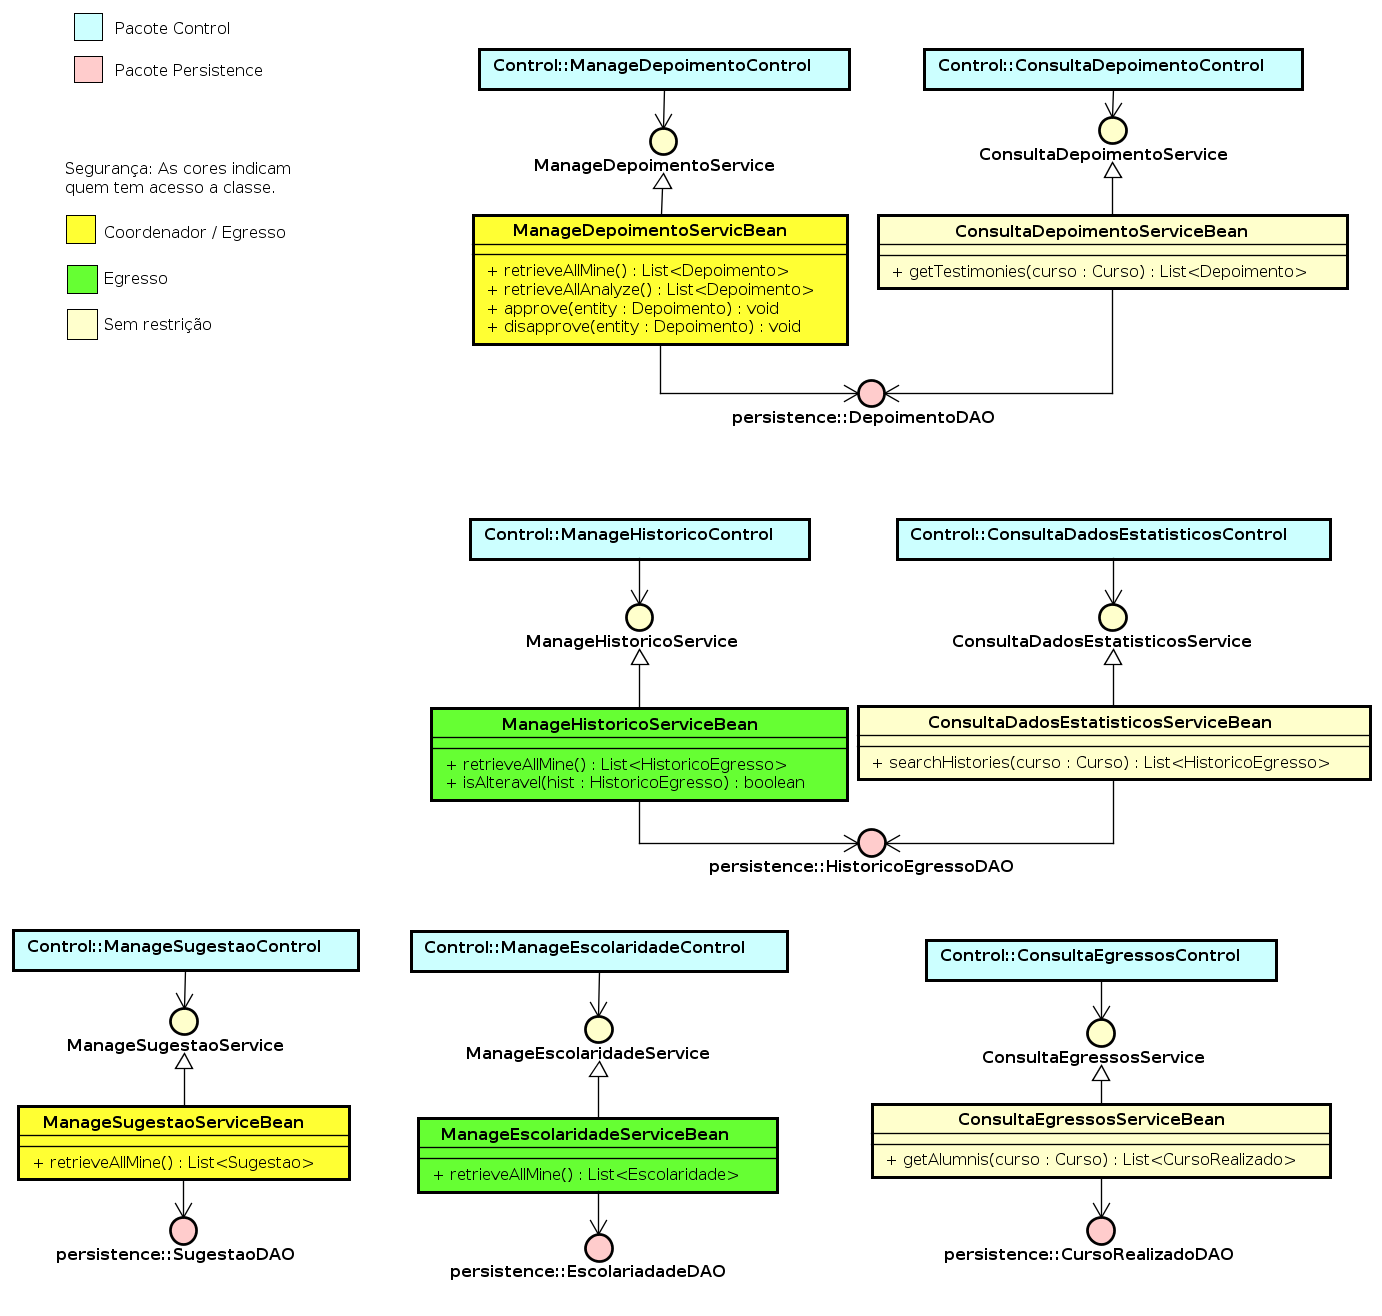
\includegraphics[width=1\textwidth]{figuras/modeloAplicacaoSugerido}
	\caption{FrameWeb Modelo de Aplicação Sugerido}
	\label{fig-modelo-aplicacao-sugerido}
\end{figure}